\documentclass[12pt]{article}
\usepackage{amsgen,amsmath,amstext,amsbsy,amsopn,amsfonts,amssymb}
\usepackage[pdftex]{graphicx}
\usepackage{hyperref}
\usepackage{graphpap}
\usepackage{url}

\title{A new method of calibrating SFTs}
\author{Vladimir Dergachev}

%% Fourier transform coefficient
\def\FTC#1#2{{\mathfrak F}_{#1}\left[#2\right]}
\def\FFTNORM{\frac{1}{\sqrt{ L}}}

\begin{document}
\maketitle
\tableofcontents
\listoffigures

\newpage
\section{General method}
\label{general_method}
The process of generating calibrated SFT can be represented as
$$
f(t)=\FFTNORM\sum_{k=-L/2}^{L/2}b_k e^{iks\omega}=\FFTNORM\sum_{k=-L/2}^{L/2}c_k R_k(t)^{-1}e^{iks\omega}
$$
where $f(t)$ is raw data, $s$ is the sample number, $L$ is the total number of samples,
 $\omega=2\pi/L$,  $b_k$ are raw SFT coefficients, $c_k$ are calibrated SFT coefficients
and $R_k(t)$ are the calibration functions:
$$
R_k(t)=\frac{1+\alpha(t)\beta(t) [C^0_kR^0_k-1]}{\alpha(t)C^0_k}
$$

The idea is that the terms $R_k(t)^{-1}e^{ikt\omega}$ represent the data we need to observe on ASQ
channel in order to produce a unit response in bin $k$ after calibration.

Let $\FTC{n}{y(t)}$ be the $n$-th Fourier coefficient:
$$
\FTC{n}{y(t)}=\FFTNORM \sum_{s=0}^{L-1}y(s)e^{-isn\omega}
$$

We compute:

\begin{equation} 
\label{gen_eqn}
\FFTNORM\sum_{k=-L/2}^{L/2}b_k R_n(t) e^{i(k-n)s\omega}=\FFTNORM\sum_{k=-L/2}^{L/2}c_k \frac{R_n(t)}{R_k(t)}e^{i(k-n)s\omega}
\end{equation}

$$
\sum_{k=-L/2}^{L/2} b_k \FTC{n-k}{R_n(t)}=\sum_{k=-L/2}^{L/2} c_k \FTC{n-k}{\frac{R_n(t)}{R_k(t)}}
$$

$$
\sum_{k=-L/2}^{L/2} b_k \FTC{n-k}{R_n(t)}=c_n+\sum_{k\neq n} c_k \FTC{n-k}{\frac{R_n(t)}{R_k(t)}}
$$

We have:
{\large
$$
\begin{array}{rcl}
\frac{R_n(t)}{R_k(t)}&=&\frac{1+\alpha(t)\beta(t) [C^0_nR^0_n-1]}{1+\alpha(t)\beta(t) [C^0_kR^0_k-1]}
    \cdot \frac{C^0_k}{C^0_n}=\\
    &=&\frac{\frac{1}{C^0_n}+\alpha(t)\beta(t)\left[R^0_n-\frac{1}{C^0_n}\right]}{
    	\frac{1}{C^0_k}+\alpha(t)\beta(t)\left[R^0_k-\frac{1}{C^0_k}\right]}=\\
    &=&\frac{C^0_k}{C^0_n}+\frac{\alpha(t)\beta(t) [C^0_nR^0_n-C^0_kR^0_k]}{1+\alpha(t)\beta(t) [C^0_kR^0_k-1]}
    \cdot \frac{C^0_k}{C^0_n}=\\
    &=&\frac{C^0_k}{C^0_n}+\frac{\alpha(t)\beta(t) \left[R^0_n-R^0_k\frac{C^0_k}{C^0_n}\right]}{\frac{1}{C^0_k}+\alpha(t)\beta(t) \left[R^0_k-\frac{1}{C^0_k}\right]}
    =\\
    &=&\frac{C^0_k}{C^0_n}+\frac{\left[R^0_n-R^0_k\frac{C^0_k}{C^0_n}\right]}{\left[R^0_k-\frac{1}{C^0_k}\right]}
        \cdot\frac{\alpha(t)\beta(t)}{
    	\frac{1}{R^0_kC^0_k-1}+\alpha(t)\beta(t)}
    =\\
    &=&\frac{C^0_k}{C^0_n}+\frac{\left[R^0_n-R^0_k\frac{C^0_k}{C^0_n}\right]}{\left[R^0_k-\frac{1}{C^0_k}\right]}
        \cdot\left[1-\frac{1}{
    	1+\alpha(t)\beta(t)[R^0_kC^0_k-1]}\right]
    \\
\end{array}
$$
}
$C^0_k$ varies from $10^{18}$ to $10^{16}$, $R^0_k$ varies from $10^{-7}$ to 
$10^{-15}$ to $10^{-18}$.

\section{Estimating $\sum_k b_k \FTC{n-k}{R_n(t)}$}

$$
\sum_k b_k \FTC{n-k}{R_n(t)}=\FTC{n}{f(t)R_n(t)}
$$

Since it is clearly inefficient to compute Fourier transform of $f(t)R_n(t)$ for each $n$
(especially as $R_n(t)$ is only known in a few points), we shall first
compute Fourier transform of $f(t)\phi_k(t)$ for a few test functions $\phi_k(t)$
and then approximate $R_n(t)$ using $\phi_k(t)$.

\subsection{Choice of $\phi_k(t)$}
Clearly, any choice of $\phi_k(t)$ that is able to provide good approximation
of $R_n(t)$ is sufficient. However, if we take into account that the size of input 
data is quite large then it is natural to request that $f(t)\phi_{k+1}(t)$ 
should be easily computable from $f(t)\phi_{k}(t)$. 

This implies that functions $\phi_{k+1}(t)/\phi_k(t)$ should have no singularities 
and, preferably, have values between $-1$ and $1$. Therefore, we adapt the following
scheme:
$$
\phi_k(t)=\left(\frac{2s-L}{L}\right)^k=\left(\phi_1(t)\right)^k
$$
Here $s$ is the sample number, $L$ is the number of samples. We set $\phi_0(t)=1$.

Another interesting choice is $\phi_1(t)=\sin\left(\frac{\pi}{2}\cdot\frac{2s-L}{L}\right)$,
$\phi_k(t)=\left(\phi_1(t)\right)^k$. For this scheme multiplication by the function $\phi_k(t)$
is equivalent to modulation of $f(t)$ by a combination of sine waves.

\subsection{Estimating $R_n(t)$}
To simplify (and speedup) computation we will estimate $R_n(t)$ as a linear
combination of $\phi_k(t)$ using least squares method.

The response curve $R_n(t)$ is available to us at specific times $t_i$, which
do not depend on $n$.

Thus:

$$
\sum_i \left(R_n(t_i)-\sum_k\alpha_k \phi_k(t_i)\right)^2\rightarrow \inf
$$

Differentiating with respect to $\alpha_{m}$ yields:
$$
\sum_i \phi_m(t_i)\left(R_n(t_i)-\sum_k\alpha_k \phi_k(t_i)\right)=0
$$

$$
\sum_k \left(\sum_i\phi_m(t_i)\phi_k(t_i)\right)\alpha_k =\sum_i\phi_m(t_i)R_n(t_i)
$$

For our choice of functions $\phi_k(t)$ we have:
$$
\sum_k \left(\sum_i\phi_1(t_i)^{k+m}\right)\alpha_k =\sum_i\phi_1(t_i)^m R_n(t_i)
$$

Let us denote by $a_k$ the sum $\sum_i \phi_1(t_i)^k$.
Then 
$$
\Phi=\left\|\sum_i\phi_1(t_i)^{k+m}\right\|_{k,m}=\left\|\sum_i a_{k+m}\right\|_{k,m}
$$
For quadratic interpolation ($\phi_0$, $\phi_1$ and $\phi_2$) with $N$ points $t_i$ we have:
$$
\begin{array}{rcl}
a_0&=&N\\
a_1&=&\sum_{i=1}^N \phi_1(t_i)\\
a_2&=&\sum_{i=1}^N \phi_1(t_i)^2\\
a_3&=&\sum_{i=1}^N \phi_1(t_i)^3\\
a_4&=&\sum_{i=1}^N \phi_1(t_i)^4\\
\end{array}
$$
and
$$
\Phi^{-1}=\frac{1}{a_0a_2a_4 -a_0a_3^2-a_1^2a_4+2a_1a_2a_3-a_2^3}
	\left\|
	\begin{array}{ccc}
	a_2a_4-a_3^2 & a_2a_3-a_1a_4 & a_1a_3-a_2^2\\
	 a_2a_3-a_1a_4 & a_0a_4-a_2^2  & a_1a_2-a_0a_3\\
	a_1a_3-a_2^2 & a_1a_2-a_0a_3 & a_0a_2 -a_1^2\\
	\end{array}
	\right\|
$$

In particular, we note that $\Phi^{-1}$ can be computed once for each SFT segment
and then $\alpha_k$ can be found by the following formula:
$$
\left\|\alpha_k\right\|_k=\Phi^{-1}\left\|\sum_i\phi_1(t_i)^mR_n(t_i)\right\|_m
$$


\section{$0$-order method}
The $0$-order approximation to $c_k$ is to assume that the term $\sum_{k\neq n} c_k \FTC{n-k}{\frac{R_n(t)}{R_k(t)}}$
vanishes. In this case we estimate
$$
\hat{c}^0_n=\FTC{n}{f(t)R_n(t)}
$$
An efficient method for computing $\hat{c}^0_n$ was discussed in the previous section.
\subsection{Reinterpretation}
The $0$-order method can be reinterpreted as following: in order to compute the
$n$-th coefficient of the calibrated SFT we assume that at each moment in time
the calibration for all frequencies is identical to the calibration of the $n$-th
bin. Then the input data can be adjusted by simply multiplying by the response
function for the $n$-th bin. The Fourier transform of the resulting data would not
have correct calibration for bins other then $n$, but we can hope to have bin $n$
calibrated correctly.

As we will show this method does produce correct calibration for bin centered
signals, however, it also produces some leakage in the neighboring bins.

\subsection{Analysis}
Suppose that the detector receives a pure wave $e^{is\omega k}$, where $s$ is the
sample number and $\omega=2\pi/L$, with $L$ being the number of samples.

Then the ASQ channel records data that has been affected by the sensitivity 
of the instrument:
$$
f(t)=R_k(t)^{-1}e^{is\omega k}
$$
We have:
$$
\hat{c}^0_n=\FTC{n}{f(t)R_n(t)}=\FTC{n}{\frac{R_n(t)}{R_k(t)}e^{is\omega k}}
$$
Thus for $n=k$ we have $\hat{c}^0_n=1$ - which is the true value. 
However for $n$ different from $k$ we have
$$
\hat{c}^0_n=\FTC{n}{\frac{R_n(t)}{R_k(t)}e^{is\omega k}}=\FTC{n-k}{\frac{R_n(t)}{R_k(t)}}
$$
The functions $R_n(t)$ are only sampled in 30 points and can be well approximated
with a quadratic polynomial. Thus the largest contribution will come from the
discontinuity in the ends of the segment. 

We will compute for the test case of linear function:
$$
\FFTNORM\int_0^{L}\frac{s}{L}e^{ism\omega}ds=-\FFTNORM\left.\frac{ism\omega-1}{Lm^2\omega^2}e^{ism\omega}\right|_0^{L}
 =-\frac{i}{m\sqrt{L}\omega}=-\frac{i\sqrt{L}}{2\pi m}
$$
Thus for a $1800$ second SFT the unit jump will contribute $0.5$ after $1$ Hz.

We note that the larger the fraction $\frac{R_n(t)}{R_k(t)}$ the bigger the leakage
into bin $n$ from bin $k$.

As an example figures \ref{h1_response_1} and \ref{h1_response_2} contain plots
of response function of H1 during S2 run.

We observe that the leakage from frequencies below $50$ Hz should be minimal and that the region
around $150$ Hz should contribute the most leakage to other bins. From the graph we see an order
of magnitude change in the response function from $150$ Hz to $550$. Thus the leakage 
from $150$ Hz region to $550$ Hz should be less than $0.5/400=1.25\cdot 10^{-3}$.


\begin{figure}
\label{h1_response_1}
\centering
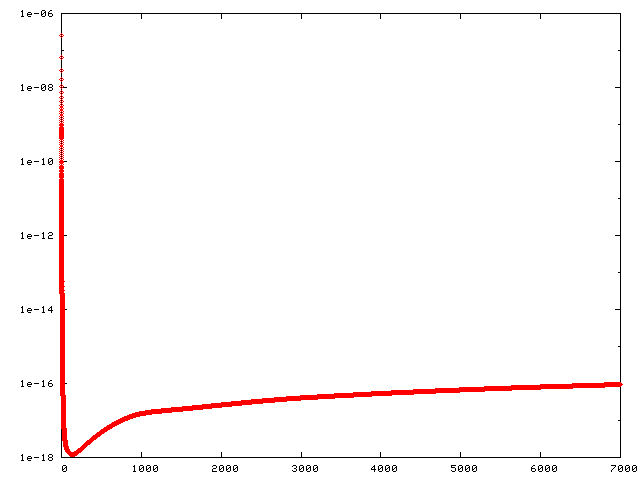
\includegraphics[scale=0.5]{S2/h1_response-1.png}
\caption{H1 response curve}
\end{figure}

\begin{figure}
\label{h1_response_2}
\centering
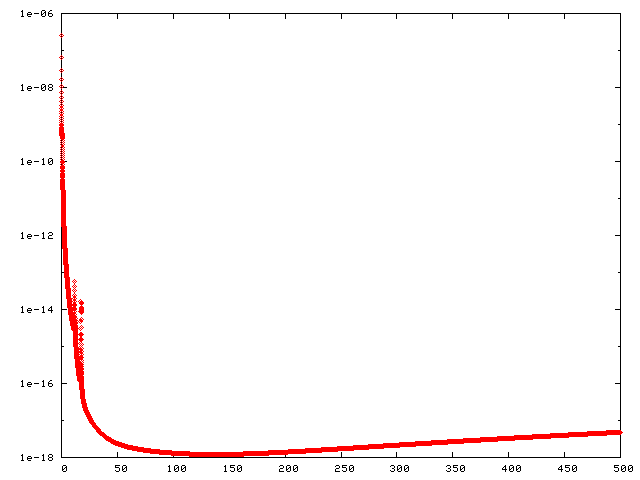
\includegraphics[scale=0.5]{S2/h1_response-3.png}
\caption{H1 response curve, small frequencies}
\end{figure}

\begin{figure}
\label{h1_cav_gain_1}
\centering
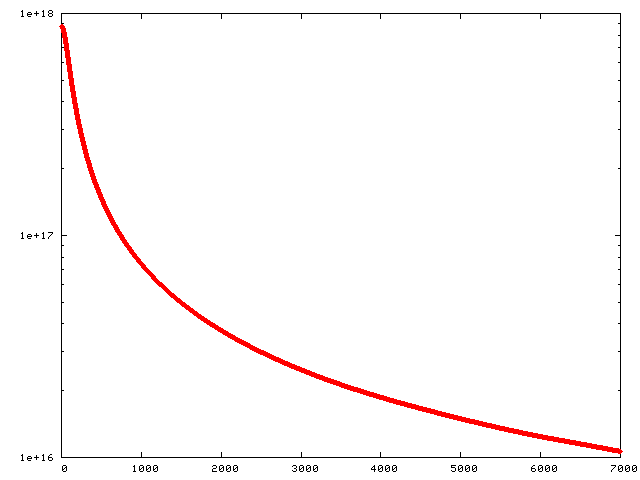
\includegraphics[scale=0.5]{S2/h1_cav_gain-1.png}
\caption{H1 CAV GAIN curve}
\end{figure}

\begin{figure}
\label{h1_cav_gain_2}
\centering
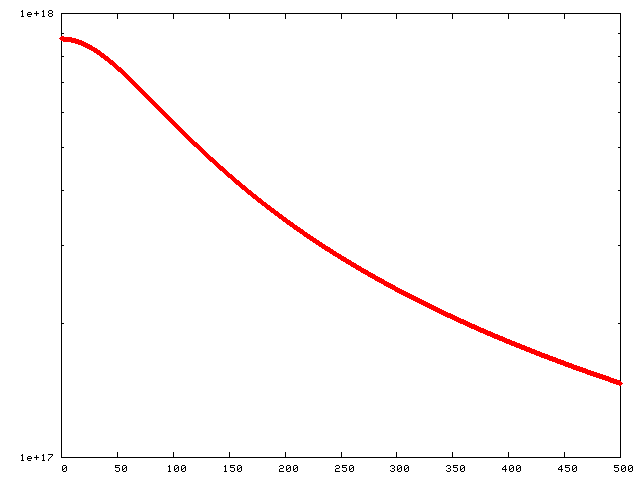
\includegraphics[scale=0.5]{S2/h1_cav_gain-3.png}
\caption{H1 CAV GAIN curve, small frequencies}
\end{figure}

\subsection{Conclusion}
$0$-order method is computationally easy, but it produces significant leakage
when $R_n(t)/R_k(t)$ is non-periodic.

\section{$1$-st order method}
The first order method is to assume that $\frac{R_n(t)}{R_k(t)}$ can be faithfully approximated
by a linear function. In other words, this method compensates leakages caused by jumps
in the end values of $\frac{R_n(t)}{R_k(t)}$.
\subsection{Derivation}
Using the formula for the general method we have:
$$
\hat{c}^0_n=\sum_{k=-L/2}^{L/2} b_k \FTC{n-k}{R_n(t)}=c_n+\sum_{k\neq n} c_k \FTC{n-k}{\frac{R_n(t)}{R_k(t)}}
$$
We estimate $\frac{R_n(t)}{R_k(t)}$ as:
$$
\frac{R_n(t)}{R_k(t)}=Const+\left(\frac{R_n(t_1)}{R_k(t_1)}-\frac{R_n(t_0)}{R_k(t_0)}\right)\frac{s}{L}
$$
where $t_0$ and $t_1$ are the end points of the segment.

Then for $n\neq k$ we have
$$
\FTC{n-k}{\frac{R_n(t)}{R_k(t)}}=-i\left(\frac{R_n(t_1)}{R_k(t_1)}-\frac{R_n(t_0)}{R_k(t_0)}\right)\frac{\sqrt{L}}{n-k}=
-i\sqrt{L}\frac{R_n(t_1)R_k(t_0)-R_n(t_0)R_k(t_1)}{R_k(t_0)R_k(t_1)(n-k)}
$$
We define operator $A$ as
$$
A_{n,k}=\left\{\begin{array}{lcl}
n=k & \qquad & 0 \\
n\neq k & \qquad & \frac{R_n(t_1)R_k(t_0)-R_n(t_0)R_k(t_1)}{(n-k)}
\end{array}
\right.
$$
Note that $A$ is symmetric.
Then we can estimate $\hat{c}^1_n$ as 
$$
\hat{c}^0_n=\hat{c}^1_n-i\sqrt{L}\sum_k A_{n,k}\frac{\hat{c}^1_k}{R_k(t_0)R_k(t_1)}
$$
Or
$$
\left\|\frac{\hat{c}^1_n}{R_n(t_0)R_n(t_1)}\right\|_n=\left(R_n(t_0)R_n(t_1)-i\sqrt{L} A\right)^{-1}\left\|\hat{c}^0_n\right\|_n
$$
\subsection{Conclusion}
$1$-st order method will compensate for leakage observed in $1$-st order method.
However, it is both memory and cpu time intensive. Large errors may accumulate
during computation of alternating sums.

\section{General method with windowing}
To mitigate the problem caused by likely non-periodicity of $R_n(t)/R_k(t)$
we will apply a windowing function $\phi$ to both sides of equation \ref{gen_eqn}:

\begin{equation} 
\label{gen_eqn}
\FFTNORM\sum_{k=-L/2}^{L/2}b_k \phi(s) R_n(t) e^{i(k-n)s\omega}=\FFTNORM\sum_{k=-L/2}^{L/2}c_k \phi(s) \frac{R_n(t)}{R_k(t)}e^{i(k-n)s\omega}
\end{equation}

After transformations similar to section \ref{general_method} we obtain:

$$
\sum_{k=-L/2}^{L/2} b_k \FTC{n-k}{\phi(s)R_n(t)}=c_n\FTC{0}{\phi(s)}+\sum_{k\neq n} c_k \FTC{n-k}{\phi(s)\frac{R_n(t)}{R_k(t)}}
$$

It is interesting to note that $c_n$ are already normalized for the power loss
introduced by the windowing function.

\section{$0$-order method with windowing}
As before, in this method we assume that the terms $\FTC{n-k}{\phi(s)\frac{R_n(t)}{R_k(t)}}$
can be neglected.

Then we estimate $\hat{c}^0_n$ as

$$
\hat{c}^0_n=\FTC{n}{f(t)\phi(s)R_n(t)}/\FTC{0}{\phi(s)}
$$

Computationally this method is equivalent to applying the windowing function
$\phi(s)$ to the time domain data $f(t)$, performing plain $0$-order estimation
method and then multiplying $\hat{c}^0_n$ by $1/\FTC{0}{\phi(s)}$.

\subsection{Analysis}
Given the input wave
$$
f(t)=R_k(t)^{-1}e^{is\omega k}
$$
the method will estimate
$$
\hat{c}^0_n=\FTC{n}{\phi(s)\frac{R_n(t)}{R_k(t)}e^{is\omega k}}/\FTC{0}{\phi(s)}=\FTC{n-k}{\phi(s)\frac{R_n(t)}{R_k(t)}}/\FTC{0}{\phi(s)}
$$
We note that for $n=k$ we get $\hat{c}^0_k=1$ - which is the true value.

The leakage into neighboring bins will depend strongly on the behaviour of $\phi(s)$ in
the ends of the segment. If we choose $\phi(s)$ as Hann or Tukey window, then
both  $\phi(s)$ and its derivative will vanish in the endpoints of the segment,
allowing us to derive the following estimate:

\if 0
$$
\begin{array}{rcl}
\FTC{n}{y(t)}&=&\FFTNORM \sum_{s=0}^{L-1}y(s)e^{-isn\omega}=\FFTNORM \sum_{s=0}^{L-1}y(s)\frac{e^{-isn\omega}-e^{-i(s+1)n\omega}}{1-e^{-in\omega}}=\\
&=&\FFTNORM \sum_{s=0}^{L-1}\frac{e^{-isn\omega}(y(s)-y(s-1))}{1-e^{-in\omega}}\approx\\
&\approx&\frac{1}{in}\FTC{n}{y'(t)}
\end{array}
$$
\fi

$$
\FTC{n-k}{\phi(s)\frac{R_n(t)}{R_k(t)}}\approx -\frac{1}{(n-k)^2}\FTC{n-k}{\phi''(s)\frac{R_n(t)}{R_k(t)}+2\phi'(s)\left(\frac{R_n(t)}{R_k(t)}\right)'+\phi(s)\left(\frac{R_n(t)}{R_k(t)}\right)''}
$$
The function $\phi''(s)\frac{R_n(t)}{R_k(t)}+2\phi'(s)\left(\frac{R_n(t)}{R_k(t)}\right)'+\phi(s)\left(\frac{R_n(t)}{R_k(t)}\right)''$
is slowly changing within the segment with a jump in the ends equal to $\phi''(0)$ times the jump $\frac{R_n(t)}{R_k(t)}$.
Thus we can use linear approximation similar to $1$-st order method to derive:
$$
\FTC{n-k}{\phi(s)\frac{R_n(t)}{R_k(t)}}\approx \frac{i\sqrt{L}}{2\pi (n-k)^3}\phi''(0)\left(\frac{R_n(t_1)}{R_k(t_1}-\frac{R_n(t_0)}{R_k(t_0)}\right)
$$
\if 0
When $\phi(s)$ is Hann its second derivative is equal to $\frac{\pi^2}{L^2}$, thus yielding a very
small leakage.
\fi

More precisily:
$$
\FFTNORM\int_0^L \frac{s}{L}\frac{1-\cos(2\pi s/L)}{2}e^{2\pi i ms/L}ds=\FFTNORM\frac{1}{8}\frac{2\pi i L (m^3-m)}{\pi^2m^2(m^2-1)^2}=\frac{i \sqrt{L}}{4 \pi m (m^2-1)}
$$
where we use $m=n-k$.

Thus a unit jump will contribute $0.43$ when $n-k=10$ and only $2\cdot 10^{-3}$ when
 $n-k=60=1/30 Hz$. See also figure \ref{leakage_0_w}

\begin{figure}
\label{leakage_0_w}
$$
\begin{array}{c|c|c}
n-k & \textrm{ Hz } & \textrm{ leakage } \\
\hline
10  &  1/180 & 0.43 \\
30  &  1/60  & 0.016 \\
60  &  1/30  & 2\cdot 10^{-3} \\
300 &  1/6   & 1.6 \cdot 10^{-5} \\
1800 & 1   & 7.4 \cdot 10^{-8} \\
\end{array}
$$
\caption{Leakage depending on bin distance for $0$-order method with windowing}
\end{figure}

{\em Note: double check estimation involving derivative, especially for missing factors.}

\subsection{Conclusion}
$0$-order method with windowing provides small leakage. An interesting property is that
windowing reduces leakage both due to non bin centered signals and to non-periodic response function
$R_n(t)$.
\end{document}
